\subsection{Guía para replicar el benchmark}

A continuación, se describe el procedimiento paso a paso para replicar el mismo benchmark utilizando el código proporcionado en el repositorio de GitHub:

\begin{enumerate}
    \item Ejecutar los algoritmos de ordenamiento y multiplicación de matrices, siguiendo las instrucciones detalladas en la sección de Experimentos. La compilación se realiza mediante \texttt{make} y la ejecución mediante los binarios generados (\texttt{./sorting} y \texttt{./matrix\_multiplication}).
    
    \item Una vez finalizada la ejecución de los algoritmos, se generarán automáticamente los archivos \texttt{bench.txt} que contienen los resultados de medición (tiempo y memoria), los cuales se almacenan en la carpeta \texttt{Data/Measurements}.
    
    \item Posteriormente, acceder a la carpeta de scripts, específicamente al directorio \texttt{plot\_generator}, y ejecutar el script de Python correspondiente fijarte que la direccion este bien puesta para la generación de gráficos. Este paso puede realizarse directamente desde la consola, siempre que los datos de medición estén disponibles.
    
    \item Las imágenes generadas se almacenarán automáticamente en el directorio \texttt{Data/plots}, listas para su inclusión en el informe final.
\end{enumerate}

\subsubsection{Algoritmos de Ordenamientos}
\begin{figure}[H]
    \centering
    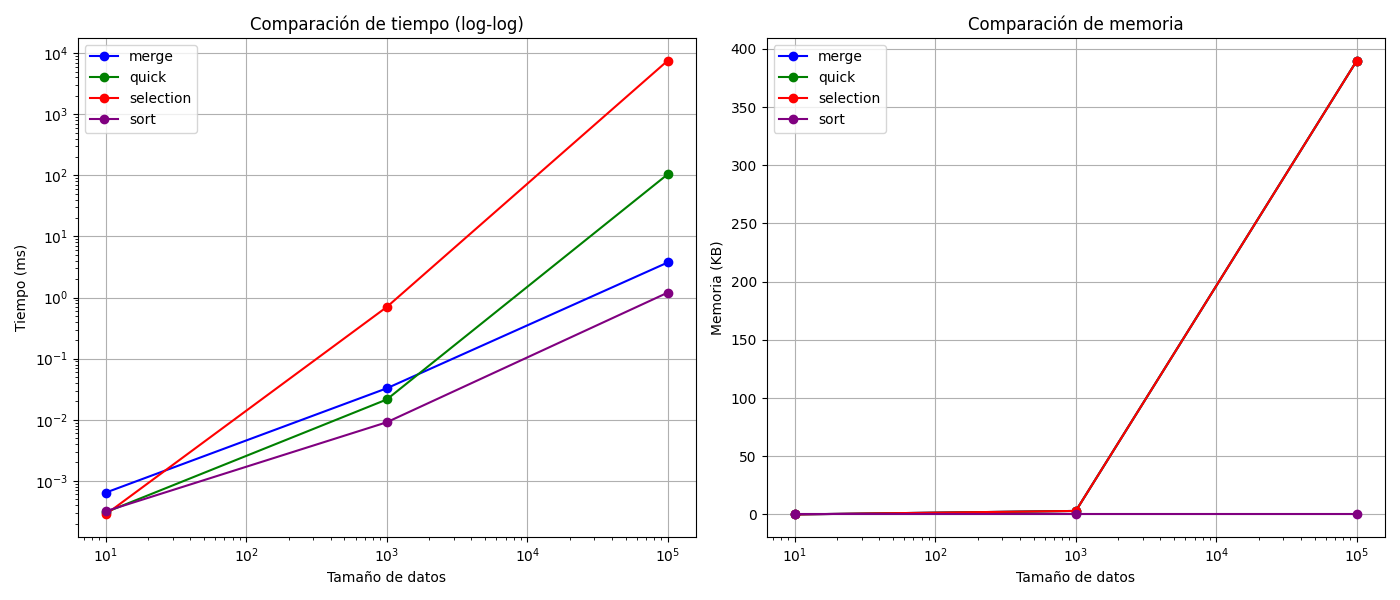
\includegraphics[width=\textwidth]{../code/sorting/data/plots/scaling_comparison.png}
    \caption{Tiempos de ejecución y memoria para algoritmos de ordenamiento.}
\end{figure}
Se observa que \textbf{Selection Sort} es el algoritmo que presenta el mayor crecimiento en el tiempo de ejecución a medida que aumenta el tamaño de la entrada, lo cual es coherente con su complejidad temporal de orden $\mathcal{O}(n^2)$. Esta tendencia se hace especialmente evidente en entradas de gran tamaño, donde su desempeño se vuelve considerablemente ineficiente en comparación con otros algoritmos.

En contraste, los algoritmos \textbf{QuickSort}, \textbf{std::sort} (de la biblioteca estándar de C++), y \textbf{MergeSort} muestran un comportamiento mucho más eficiente, gracias a sus complejidades temporales promedio de $\mathcal{O}(n \log n)$. Entre ellos, \textbf{QuickSort} exhibe una ligera desventaja en ciertos casos particulares, dado que puede alcanzar su peor caso de complejidad $\mathcal{O}(n^2)$ en situaciones específicas, como entradas ya ordenadas o altamente desbalanceadas, si no se implementan estrategias de pivoteo adecuadas.

No obstante, en el escenario general evaluado, \textbf{QuickSort} y \textbf{std::sort} se comportaron de manera muy competitiva, validando su aplicabilidad práctica en una amplia gama de problemas de ordenamiento. De manera destacada, \textbf{std::sort} se consolidó como el algoritmo más eficiente en nuestras mediciones, superando ligeramente a \textbf{MergeSort}. Esta ventaja se debe a que \texttt{std::sort} implementa una combinación optimizada de \texttt{QuickSort}, \texttt{HeapSort} y \texttt{InsertionSort}, conocida como \textit{Introsort}, lo que le permite adaptarse dinámicamente al patrón de la entrada y minimizar el tiempo de ejecución en la mayoría de los casos prácticos. Aunque \textbf{MergeSort} ofrece una garantía teórica de $\mathcal{O}(n \log n)$ en todos los casos, su sobrecarga de memoria adicional y operaciones de copia lo hacen marginalmente menos competitivo que \textbf{std::sort} en ambientes de alto rendimiento como el evaluado.
\\
En cuanto al consumo de memoria, se observa que todos los algoritmos de ordenamiento analizados (\textbf{std::sort}, \textbf{Selection Sort}, \textbf{QuickSort} y \textbf{MergeSort}) presentan un uso muy acotado de memoria adicional respecto al tamaño de las entradas procesadas.

De acuerdo a las mediciones obtenidas, para instancias de tamaño pequeño (10 a 1000 elementos), la memoria utilizada se mantuvo en torno a los 0 a 3 KB, mientras que para entradas de tamaño 100,000 elementos, el consumo de memoria alcanzó aproximadamente los 390 KB. Estos valores reflejan un comportamiento prácticamente lineal en la relación entre el tamaño del input y la memoria ocupada.

El \textbf{std::sort} de la biblioteca estándar de C++ destacó por su mínima utilización de memoria adicional, aprovechando que su implementación basada en \textit{Introsort} opera principalmente de manera \textit{in-place} en memoria, requiriendo sólo una sobrecarga constante. 

En contraste, \textbf{MergeSort} presentó un consumo similar de memoria, aunque su naturaleza intrínseca requiere la creación de arreglos temporales para realizar las operaciones de mezcla, lo que podría penalizar su eficiencia espacial en aplicaciones donde el uso de memoria sea crítico.

Por su parte, \textbf{Selection Sort} y \textbf{QuickSort} también mantuvieron un perfil de consumo de memoria bajo, acorde a sus implementaciones clásicas que, en su mayoría, modifican el arreglo original sin recurrir a estructuras auxiliares adicionales.

En general, los resultados experimentales evidencian que todos los algoritmos implementados son altamente eficientes en términos de uso de memoria, manteniéndose dentro de márgenes prácticos para sistemas modernos incluso con volúmenes de datos elevados.
\\
Para una mejor visualización de las diferencias en el comportamiento de los algoritmos de ordenamiento en términos de tiempo de ejecución y consumo de memoria, se presentan gráficos individuales en el Apéndice (ver Figuras \ref{fig:scaling_sort} a \ref{fig:scaling_merge}). Esta separación permite observar de manera más clara cómo varía la eficiencia de \texttt{std::sort}, \texttt{QuickSort}, \texttt{Selection Sort} y \texttt{MergeSort} conforme aumenta el tamaño de la entrada.

\subsubsection{Multiplicación de Matrices}
\begin{figure}[H]
    \centering
    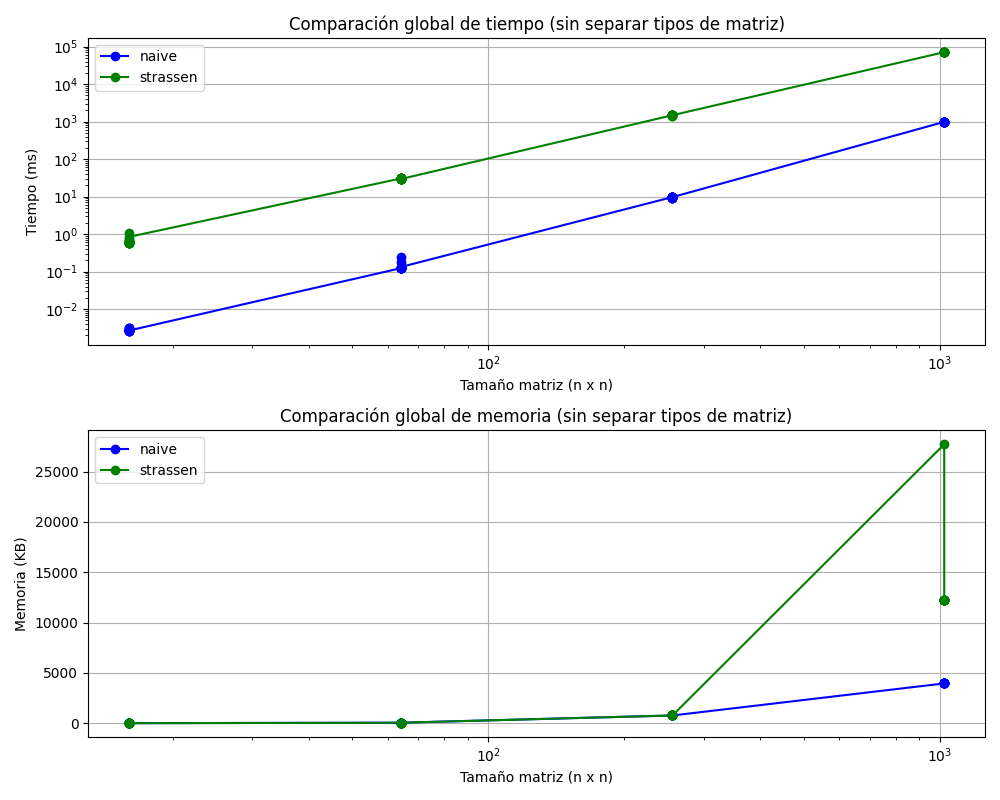
\includegraphics[width=\textwidth]{../code/matrix_multiplication/data/plots/comparacion_global_algoritmos.png}
    \caption{Comparación de tiempos y memoria para métodos de multiplicación de matrices.}
\end{figure}
En el caso de los algoritmos de multiplicación de matrices, se observaron diferencias notables tanto en consumo de memoria como en tiempo de ejecución entre el método \textbf{Naive} y el método de \textbf{Strassen}.

En cuanto al consumo de memoria, el algoritmo \textbf{Naive}, basado en el enfoque tradicional de triple bucle anidado, presentó un uso muy controlado de recursos. Para matrices de tamaño $1024 \times 1024$, el consumo de memoria fue de aproximadamente 3956 KB, mientras que en tamaños pequeños como $16 \times 16$ se mantuvo en apenas 3 KB. Esto se debe a que \textbf{Naive} trabaja directamente sobre los arreglos de entrada y el arreglo resultado, sin necesidad de generar estructuras auxiliares adicionales.

Por otro lado, el método de \textbf{Strassen} evidenció un consumo de memoria mucho mayor, alcanzando alrededor de 12,288 KB para matrices de $1024 \times 1024$. Esto se explica porque \textbf{Strassen} requiere múltiples submatrices en cada nivel de recursión para realizar las combinaciones de sumas, restas y productos parciales, lo que incrementa sustancialmente su demanda de memoria.

Respecto al tiempo de ejecución, se registró que \textbf{Naive} fue consistentemente más rápido que \textbf{Strassen} en todos los tamaños de matrices analizados. Por ejemplo, para instancias de $1024 \times 1024$, \textbf{Naive} completó las operaciones en aproximadamente 970 ms, mientras que \textbf{Strassen} tardó más de 70,000 ms (alrededor de 70 segundos), evidenciando una diferencia de dos órdenes de magnitud.

Este resultado contrasta con la expectativa teórica de que \textbf{Strassen}, con una complejidad asintótica de $\mathcal{O}(n^{\log_2 7}) \approx \mathcal{O}(n^{2.81})$, debería superar a \textbf{Naive} ($\mathcal{O}(n^3)$) para tamaños de matrices muy grandes. Sin embargo, debido al considerable overhead de operaciones adicionales (sumas y restas de submatrices) y gestión intensiva de memoria intermedia, el algoritmo \textbf{Strassen} no siempre se ve beneficiado por las arquitecturas modernas de los computadores. Esto se debe a la sobrecarga en operaciones de suma y el manejo de submatrices, que no siempre aprovechan de manera óptima el acceso eficiente a la memoria cache, ni se adaptan fácilmente a las técnicas de paralelización, factores que juegan un papel fundamental en el rendimiento práctico en hardware contemporáneo.

En resumen, para los tamaños de entrada considerados en este informe, \textbf{Naive} no solo fue más eficiente en consumo de memoria, sino que además obtuvo tiempos de ejecución notablemente menores que \textbf{Strassen}, posicionándose como la opción preferente en escenarios de matrices de tamaño moderado.
